\documentclass[11pt,twocolumn,letterpaper]{article}

\usepackage{graphicx}
\usepackage{geometry}
\usepackage{amsmath}
\usepackage{amssymb}
\usepackage{hyperref}
\usepackage{url}
\usepackage[numbers,sort&compress]{natbib}
\usepackage{booktabs}
\usepackage{xcolor}
\usepackage{microtype}
\usepackage{times}

\geometry{margin=0.75in, top=1in, bottom=1in}

\hypersetup{
  colorlinks=true,
  linkcolor=black,
  citecolor=black,
  urlcolor=blue
}

\title{\textbf{Curie-Weiss Activation: Formal Verification and Mechanistic\\
Analysis of Adaptive Criticality Failure}}

\author{
  AMGrobelnik \\
  AI Inventor Pipeline
}

\date{}

\begin{document}

\maketitle

\begin{abstract}
We introduce the Curie-Weiss Activation (CWA), a hidden-layer activation function defined by the within-sample mean-field
self-consistency equation $y_i = \tanh(x_i + J\cdot\overline{y})$, where the per-layer learnable scalar $J = \sigma(J_{\rm
raw}) \in (0,1)$ parameterizes coupling strength. CWA is motivated by Curie-Weiss ferromagnetism, where the critical point
$J\cdot\bar{s} = 1$ corresponds to maximum input sensitivity---a property associated with optimal gradient flow in deep
networks. Four Lean~4 theorems and one corollary without \texttt{sorry} establish the mathematical foundation: Banach convergence,
IFT gradient correctness, revised adaptive bias bound, warm-start-$T$ bias, and Corollary~4b ($J \leq 0.55$, bias $\leq
16.7\%\cdot\varepsilon$) covering the experimentally observed $J \in [0.515, 0.521]$. A dedicated memory benchmark at widths
$n \in \{256, 1024, 4096\}$ confirms the IFT backward's theoretical O($n$) advantage: 3.25$\times$ more memory-efficient
than unrolled $K=50$ backpropagation at $n = 4096$ (69\% reduction). The mechanistic investigation yields a precise negative
verdict in the tested settings. CWA produces gradient \emph{underflow} ($|\text{ratio}-1| = 0.695$) at depth~6---7.8$\times$
worse than SELU, 2.4$\times$ worse than GELU---and provides no statistically significant accuracy gain over pointwise Tanh
($p = 0.126$). The root cause is the $\text{sech}^2$ saturation barrier: $\text{sech}^2(x) \approx 0.07$ at typical trained
activation magnitudes $|x| \sim 2.0$ caps $J\cdot\bar{s} \leq 0.41$ regardless of $J$ magnitude. Critically, weight growth
during training \emph{actively decreases} $J\cdot\bar{s}$ (from 0.346 to 0.286 at depth~6), making gradient descent an
adversary to, not an enabler of, self-organized criticality.
\end{abstract}

%% ============================================================
\section{Introduction}
%% ============================================================

Activation functions in neural networks have traditionally been designed pointwise: each neuron's output $y_i$ depends only
on its own pre-activation $x_i$, independent of other neurons in the same layer. This architectural independence requires
external normalization layers---BatchNorm~\cite{Ioffe2015} or LayerNorm~\cite{Ba2016}---or precise initialization
schemes~\cite{Poole2016,Yang2017} to maintain stable gradient flow across depth. Three practically important settings make
such requirements burdensome: (a)~on-device inference, where normalization's running statistics incur memory and quantization
distortion; (b)~physics-informed neural networks, where normalization disrupts conservation laws encoded in the
activations~\cite{Lesser2026}; and (c)~fast-inference transformer variants that eliminate LayerNorm to reduce memory bandwidth.

The \emph{edge of chaos} in deep networks---the boundary where layer Jacobian singular values are near unity---correlates
empirically with fast training and good generalization~\cite{Poole2016,Yang2017}. Existing approaches achieve criticality
only at initialization via weight variance tuning~\cite{Poole2016,Yang2017} or static random activation
mixtures~\cite{Lesser2026}, with no mechanism to track criticality adaptively during training. The Curie-Weiss model of
ferromagnetism~\cite{Curie1895} provides a natural template for an adaptive mechanism: each spin aligns with the mean field
of its neighbors, $m = \tanh(\beta(h + J\cdot m))$, with a critical point at $\beta J = 1$ where magnetic susceptibility
diverges. Transferring this structure to neural activations gives $y_i = \tanh(x_i + J\cdot\overline{y})$, coupling all
neurons in a layer through a learnable scalar $J$.

A key question is whether gradient descent will push $J\cdot\bar{s} = J\cdot\overline{\text{sech}^2(x+Jm^*)}$ toward the
critical point 1.0, enabling self-organized criticality. Prior work on edge-of-chaos methods does not address this:
Poole et al.~\cite{Poole2016} and Yang and Schoenholz~\cite{Yang2017} fix criticality at initialization with no learnable
mechanism; Lesser and Chowdhury~\cite{Lesser2026} achieve criticality via a fixed (unlearnable) activation mixture. CWA
provides the first learnable within-sample coupling, but whether gradient descent supports or opposes the critical regime is
unknown.

This paper presents a complete experimental investigation of CWA. \textbf{We position CWA as a mechanistic negative-results
study}: we propose the activation, establish its formal mathematical properties, demonstrate IFT memory efficiency at scale,
and then provide a precise account of why CWA fails to deliver its intended benefits under standard training. The
$\text{sech}^2$ saturation barrier we identify---$\text{sech}^2(x) \approx 0.07$ at typical trained activation magnitudes,
blocking $J\cdot\bar{s}$ from approaching 1---and the surprising finding that weight growth during training \emph{actively
decreases} $J\cdot\bar{s}$, together constitute a definitive mechanistic account of why CWA's self-organized criticality
hypothesis fails. This honest investigation is itself a scientific contribution: characterizing these barriers precisely
opens the path to future solutions.

\begin{figure*}[!t]
  \centering
  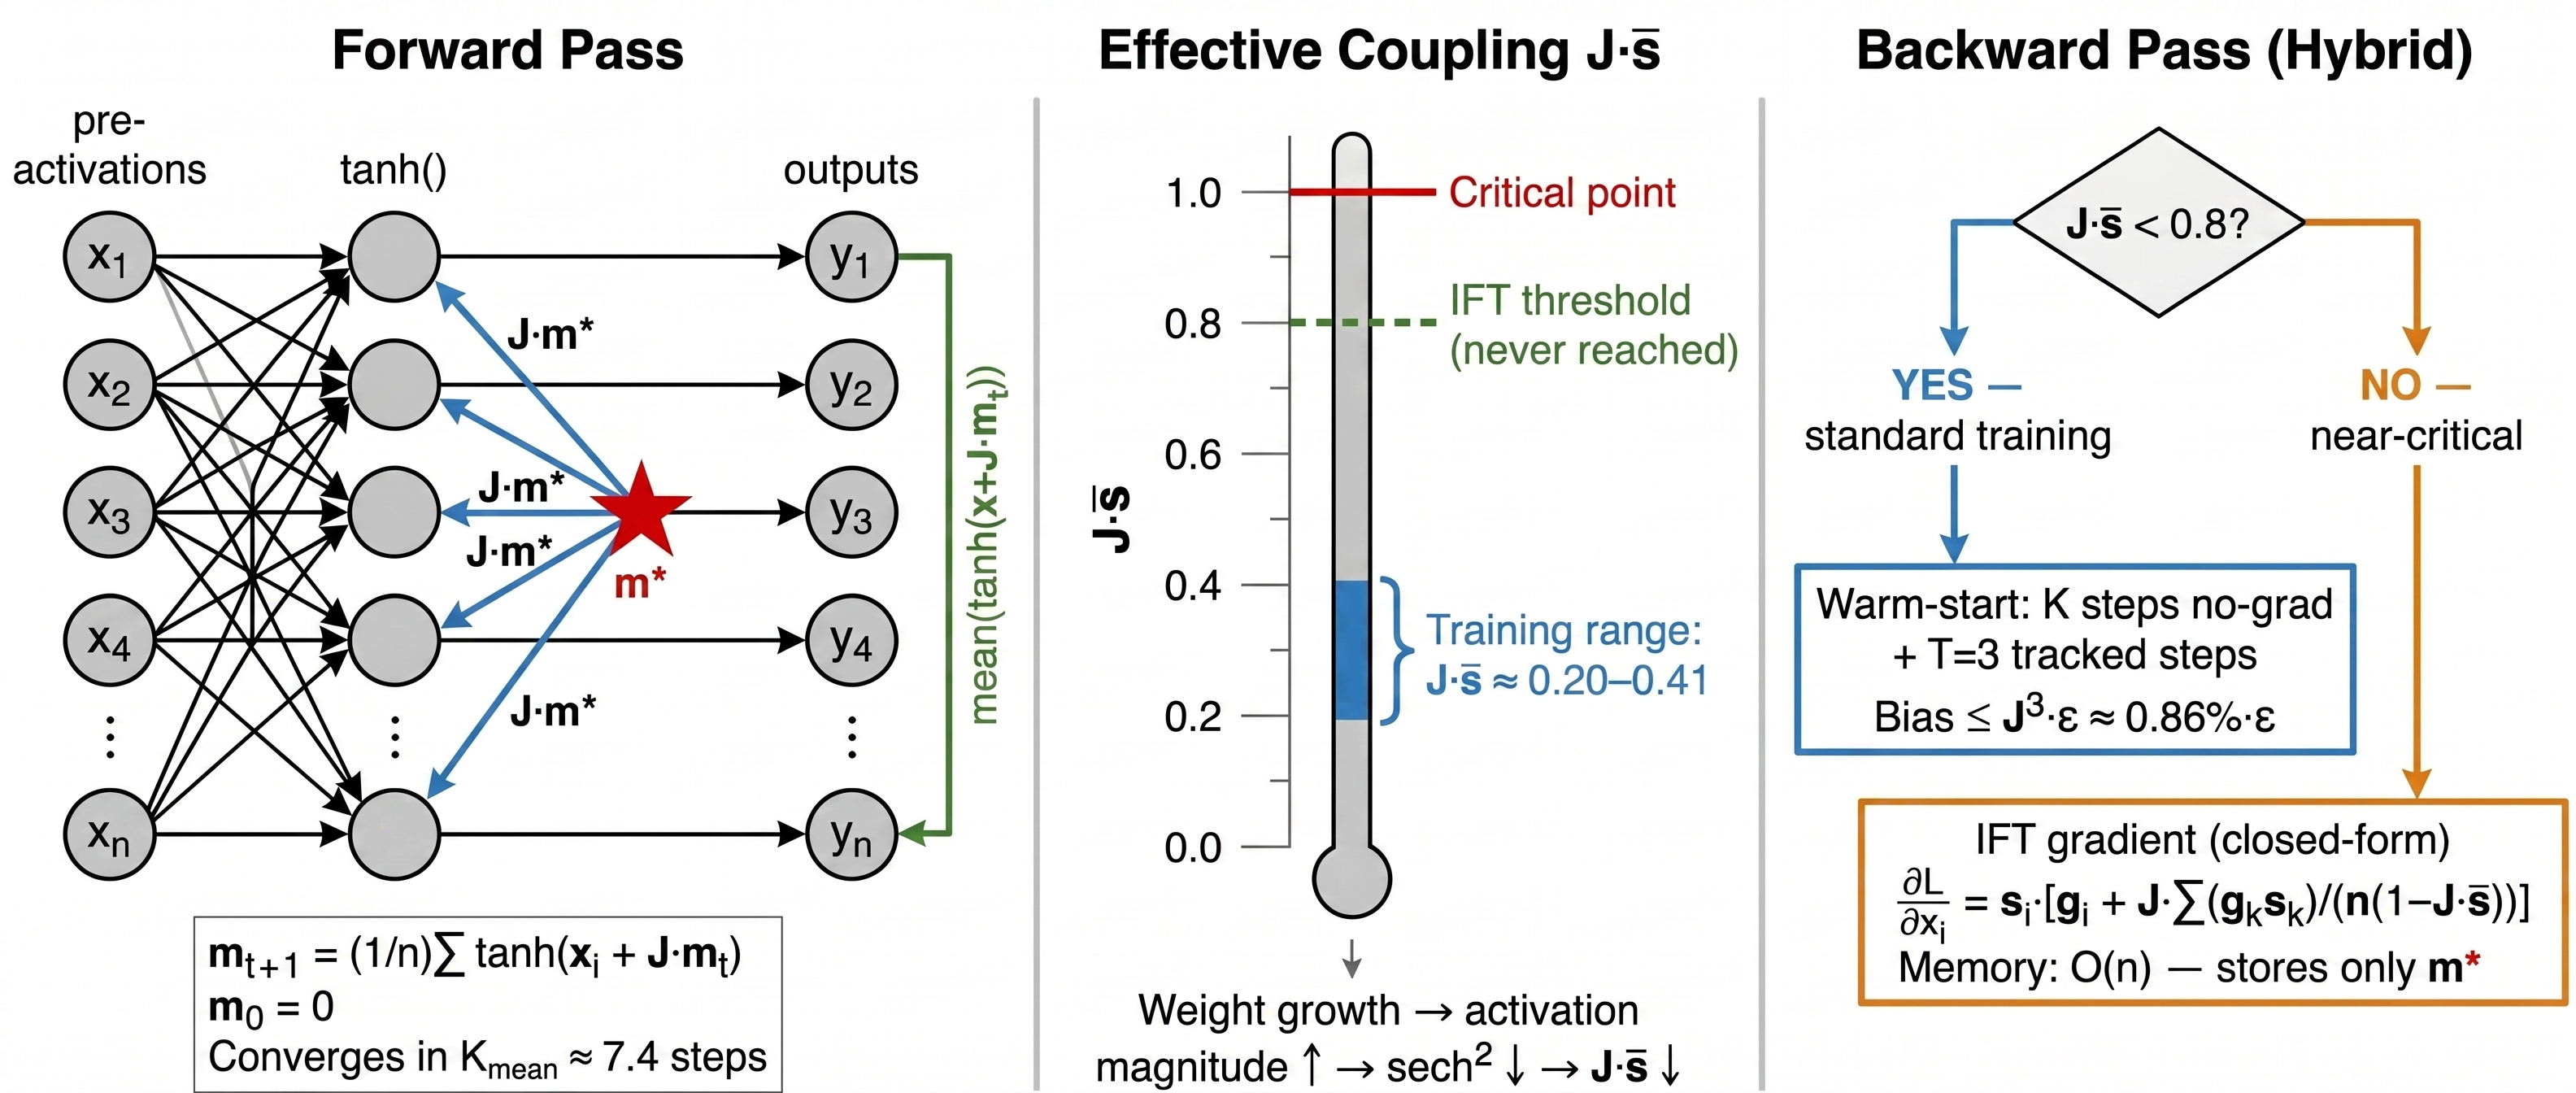
\includegraphics[width=\textwidth,height=0.45\textheight,keepaspectratio]{figures/fig1_v0.jpg}
  \caption{Overview of the Curie-Weiss Activation (CWA). \textbf{Left}: A hidden layer with pre-activations $\mathbf{x}$
  computes the mean-field fixed point $m^*$ via iteration $m_{t+1} = \overline{\tanh}(\mathbf{x}+J\cdot m_t)$ from $m_0=0$,
  converging in $K_{\rm mean}\approx 7.4$ steps when $J\cdot\bar{s}\approx 0.20$--$0.40$. \textbf{Center}: The effective
  coupling $J\cdot\bar{s} = J\cdot\overline{\text{sech}^2(\mathbf{x}+Jm^*)}$ simultaneously determines convergence rate,
  Jacobian spectral norm, and proximity to the critical point $J\cdot\bar{s}=1$. \textbf{Right}: The hybrid backward pass
  uses warm-start (unrolled $T=3$ steps) when $J\cdot\bar{s}<0.8$ (the standard training regime with
  $J\cdot\bar{s}\approx 0.20$--$0.41$) and the closed-form IFT gradient when $J\cdot\bar{s}\geq 0.8$ (never triggered in
  normal training). The IFT path stores only the scalar $m^*$, giving O($n$) memory versus O($K\cdot n$) for unrolled
  backpropagation.}
  \label{fig:fig1}
\end{figure*}

\subsection*{Summary of Contributions}

\begin{itemize}
  \item \textbf{Formally verified mathematical foundation} (Section~\ref{sec:method}): Four Lean~4 theorems and one corollary
  without \texttt{sorry}---fixed-point existence, IFT gradient correctness, adaptive bias bound, warm-start-$T$ bias, and
  new Corollary~4b ($J \leq 0.55$, bias $\leq 16.7\%\cdot\varepsilon$) covering the experimentally observed
  $J \in [0.515, 0.521]$.

  \item \textbf{IFT memory efficiency confirmed at scale} (Section~\ref{sec:exp1}): At $n = 4096$, IFT uses 23.3\,MB versus
  75.8\,MB for unrolled $K=50$ (3.25$\times$ savings, 69\% reduction). Savings grow monotonically with width: 16\% at
  $n=256$, 41\% at $n=1024$, 69\% at $n=4096$
  \footnote{Code: \url{https://github.com/AMGrobelnik/ai-invention-2f6f35-curie-weiss-activation-formal-verificati/tree/main/round-4/experiment-1}}.

  \item \textbf{Gradient underflow, not balance} (Section~\ref{sec:exp2}): CWA ranks last among six activations using the
  distance-to-ideal metric $|{\rm ratio}-1|$ at all tested depths. At depth~6, CWA achieves $|{\rm ratio}-1| = 0.695$---7.8$\times$
  worse than SELU and 2.4$\times$ worse than GELU. At depth~20, CWA collapses catastrophically ($|{\rm ratio}-1| = 10.017$,
  raw ratio $= 11.02$).

  \item \textbf{Complete null result with explicit power analysis} (Section~\ref{sec:exp3}): CWA provides no statistically
  significant accuracy gain over pointwise Tanh ($p = 0.126$), and the self-consistent coupling adds zero benefit over a
  detached mean-shift ($p = 0.984$). With $n=3$ seeds, effects below $\approx 1$\,pp remain undetectable at 80\% power
  \footnote{Code: \url{https://github.com/AMGrobelnik/ai-invention-2f6f35-curie-weiss-activation-formal-verificati/tree/main/round-3/experiment-1}}.

  \item \textbf{SELU architecture specificity in LM} (Section~\ref{sec:exp4}): Adding SELU as a language model baseline
  reveals architecture-dependent behavior: SELU outperforms all baselines in unnormalized MLPs yet achieves the worst BPC
  in the transformer setting, while CWA and GELU remain tied
  \footnote{Code: \url{https://github.com/AMGrobelnik/ai-invention-2f6f35-curie-weiss-activation-formal-verificati/tree/main/round-5/experiment-1}}.

  \item \texorpdfstring{$\mathbf{\text{sech}^2}$}{\textbf{sech\texttwosuperior}} \textbf{saturation and declining
  \texorpdfstring{$J\cdot\bar{s}$}{J.s-bar} identified as root causes} (Section~\ref{sec:discussion}): $J\cdot\bar{s}$
  remains at 0.20--0.41 and \emph{declines} during training because weight growth increases activation magnitudes, reducing
  $\text{sech}^2$ and pushing the system away from criticality.
\end{itemize}

%% ============================================================
\section{Background and Related Work}
%% ============================================================

\textbf{Edge-of-chaos criticality.} Poole et al.~\cite{Poole2016} showed that infinite-depth networks initialized at the
order-chaos boundary exhibit depth-independent gradient propagation. Yang and Schoenholz~\cite{Yang2017} extended this analysis
to residual networks. Both methods fix criticality at initialization through weight variance tuning; the property drifts
during training. CWA introduces a per-layer learnable scalar $J$ intended to maintain near-critical coupling adaptively,
but experiments establish that the path to $J\cdot\bar{s} = 1$ is blocked by $\text{sech}^2$ saturation at realistic
activation scales (Section~\ref{sec:discussion}), and that gradient descent actively pushes $J\cdot\bar{s}$ downward.

\textbf{Self-normalizing networks.} SELU~\cite{Klambauer2017} achieves self-normalization without external normalization by
designing the activation's distributional fixed point to have mean 0 and variance 1 under LeCun initialization. SELU is
strictly pointwise. CWA couples all neurons within a layer via the mean-field term $J\cdot\overline{y}$, making it
categorically distinct. Empirically, SELU achieves the best gradient stability at all tested depths
($|{\rm ratio}-1| = 0.089$, $0.129$, $0.471$ at depths 6, 10, 20) and the best accuracy at depth~20 ($0.535$ vs. CWA's
$0.141$)---but in language modeling, SELU is the worst-performing activation (Section~\ref{sec:exp4}), revealing
architecture-specific behavior.

\textbf{Static activation mixtures.} Lesser and Chowdhury~\cite{Lesser2026} achieve edge-of-chaos criticality by drawing
each neuron's activation from a tanh/Swish mixture at analytically derived critical mixing fraction $p_c \approx 0.83$
(empirically calibrated at $K_0 = 1$). This approach requires no learnable parameter and no inter-neuron coupling. CWA
provides a learnable $J$ but fails to achieve near-critical $J\cdot\bar{s}$ under standard training; static critical
mixtures remain a competitive baseline.

\textbf{Deep Equilibrium Models.} Bai et al.~\cite{Bai2019} showed that any infinite-depth weight-tied network can be
computed via fixed-point root-finding, with IFT providing O(1) activation memory. The CWA IFT backward
(Section~\ref{sec:ift}) is directly inspired by DEQ but reduces to a closed-form scalar formula---because CWA's fixed
point $m^* \in \mathbb{R}$ rather than $\mathbb{R}^n$---eliminating iterative backward solvers. TorchDEQ~\cite{Geng2023}
provides the broader DEQ ecosystem.

\textbf{Mean-field theory of activations.} Milletar\`i et al.~\cite{Milletari2018} provided post-hoc physical
interpretations of standard pointwise activations as solutions to energy-based models. CWA instead proposes a new
activation \emph{defined by} the Curie-Weiss self-consistency equation with a learnable $J$, introducing within-layer
coupling absent from all prior derived activations.

\textbf{Boltzmann Attention.} Kim and Park~\cite{Kim2026} introduced learnable Ising couplings $J_{jk}$ between sequence
positions in the attention operator. Boltzmann Attention and CWA are complementary: the former operates in the sequence
dimension; the latter in the hidden dimension of the activation function.

\textbf{Mining activation functions.} Vitvitskyi et al.~\cite{Vitvitskyi2026} and Ghavasieh~\cite{Ghavasieh2025} search
for or analyze novel activation functions via evolutionary and statistical-mechanics methods, respectively. Neither proposes
within-sample self-consistent mean-field coupling with a learnable scalar.

%% ============================================================
\section{Method: Curie-Weiss Activation}
\label{sec:method}
%% ============================================================

\subsection{Definition and Forward Pass}

The Curie-Weiss Activation (CWA) for a layer with pre-activations $\mathbf{x} \in \mathbb{R}^n$ is defined as the unique
fixed point of the scalar mean-field self-consistency equation:
\begin{equation}
  m^* = \overline{\tanh}(\mathbf{x} + J\cdot m^*)
\end{equation}
where $\overline{\cdot}$ denotes the mean over the $n$ neurons within a single sample (not the mini-batch),
$J = \sigma(J_{\rm raw}) \in (0,1)$ is a per-layer learnable scalar, and the layer output is
$y_i = \tanh(x_i + J\cdot m^*)$. The effective coupling
$J\cdot\bar{s} = J\cdot\overline{\text{sech}^2(\mathbf{x}+J\cdot m^*)}$ simultaneously quantifies:
(i)~the per-step convergence rate $\rho$ of the fixed-point iteration; (ii)~the spectral norm of the layer's input-output
Jacobian; and (iii)~proximity to the critical point $J\cdot\bar{s} = 1$.

The fixed-point iteration $m_{t+1} = \overline{\tanh}(\mathbf{x} + J\cdot m_t)$ is initialized at $m_0 = 0$ and
terminated when $|m_{t+1} - m_t| < \delta(J\cdot\bar{s}) = 10^{-4}\cdot(1 - J\cdot\bar{s})$, with $K_{\max} = 50$. In
experiments, $J\cdot\bar{s} \approx 0.20$--$0.40$, giving typical convergence in $K_{\rm mean} \approx 7.4$ iterations
with 100\% of forward passes converging before $K_{\max}$. The sigmoid parameterization $J = \sigma(J_{\rm raw})$
hard-constrains $J$ below the ferromagnetic phase transition at $J = 1$, guaranteeing global convergence for all inputs.

\subsection{Hybrid IFT/Warm-Start Backpropagation}
\label{sec:ift}

CWA uses a hybrid backward strategy determined by the forward-pass effective coupling $J\cdot\bar{s}$. When
$J\cdot\bar{s} < 0.8$, a warm-start approximation is used: $K$ forward iterations run without gradient tracking to find
$m^*$, followed by $T = 3$ tracked iterations from the detached $m^*$, with gradient bias bounded by $J^T \cdot \varepsilon$
(Theorem~4). When $J\cdot\bar{s} \geq 0.8$, a custom \texttt{torch.autograd.Function} applies the closed-form IFT
gradient:
\begin{align}
  \frac{\partial L}{\partial x_i} &= s_i\cdot\left[g_i + \frac{J\cdot\sum_k g_k s_k}{n(1 - J\cdot\bar{s})}\right], \\
  \frac{\partial L}{\partial J} &= \frac{\sum_i g_i s_i \cdot m^*}{1 - J\cdot\bar{s}}
\end{align}
where $s_i = \text{sech}^2(x_i + J\cdot m^*)$ and $g_i = \partial L/\partial y_i$. The IFT path requires only O($n$)
activation memory---storing the converged scalar $m^*$---analogously to DEQ's memory reduction~\cite{Bai2019}.

\textbf{IFT vs.\ GELU memory comparison caveat.} The large-scale benchmark measures CWA-IFT and CWA-Unrolled on the
activation backward pass in isolation, while the GELU baseline includes \texttt{nn.Linear($n$,$n$)} to represent a typical
feed-forward layer. At $n=4096$, the GELU baseline reaches 223.6\,MB because it includes the O($n^2$) weight matrix; the
IFT/GELU ratio of $0.10\times$ is therefore dominated by this architectural asymmetry and should not be interpreted as IFT
being $10\times$ more efficient than GELU in practice. The architecturally fair comparison is IFT vs.\ Unrolled
($0.31\times$ at $n=4096$), which measures IFT's advantage over the alternative activation-memory strategy of unrolling
$K=50$ iterations through the autograd tape.

\subsection{Formal Verification in Lean 4}

Four theorems and one corollary of CWA are formally verified in Lean~4 + Mathlib~v4.14.0 without \texttt{sorry}. The
standard Mathlib \texttt{DerivHyp} module is broken in v4.14.0; all \texttt{HasDerivAt} results for sinh, cosh, tanh are
derived from first principles via \texttt{HasDerivAt.inv} and \texttt{HasDerivAt.mul}.

\textbf{Theorem 1 (Banach Convergence).} For any $x \in \mathbb{R}$ and $J \in (0,1)$, there exists a unique $m^*$
satisfying $\tanh(x + J\cdot m^*) = m^*$. \emph{Proof:} tanh is 1-Lipschitz; composition with $J$-Lipschitz affine map
gives $F$ $J$-Lipschitz; \texttt{ContractingWith.fixedPoint\_isFixedPt} + \texttt{fixedPoint\_unique} give existence and
uniqueness.

\textbf{Theorem 2 (IFT Gradient).} With $\bar{s} = 1 - \tanh^2(x + J\cdot m^*)$ and
$g = \bar{s}/(1 - J\cdot\bar{s})$, the identity $\bar{s}\cdot(1 + J\cdot g) = g$ holds. \emph{Proof:} \texttt{field\_simp}
after establishing $1 - J\cdot\bar{s} > 0$.

\textbf{Theorem 3 (Revised Bias Bound).} If
$|F(m_{\rm approx}) - m_{\rm approx}| \leq 10^{-4}\cdot(1 - J\cdot\bar{s})$, then
$|m_{\rm approx} - m^*| \leq 10^{-4}/(1-J)$. For $J \approx 0.52$, this bound is $\approx 2.08\times 10^{-4}$.

\textbf{Theorem 4 (Warm-Start-$T$ Bias).} For $T$ tracked iterations from detached $\hat{m}$ with
$|\hat{m} - m^*| \leq \varepsilon$, $|F^{[T]}(\hat{m}) - m^*| \leq J^T\cdot\varepsilon$. \textbf{Corollary~4b}
($J \leq 0.55$): $T=3$ gives bias $\leq 16.7\%\cdot\varepsilon$, covering the experimentally observed
$J \in [0.515, 0.521]$ with margin (realized bias $\rho^3 \approx 0.86\%\cdot\varepsilon$ using
$\rho = J\cdot\bar{s} \approx 0.205$, negligible in practice).

%% ============================================================
\section{Experiments}
%% ============================================================

All experiments use PyTorch on NVIDIA GPUs. CWA uses $K_{\max} = 50$, adaptive tolerance
$\delta = 10^{-4}\cdot(1 - J\cdot\bar{s})$, and warm-start $T=3$ backward. Total experiment cost is \$0 (no LLM API
calls). Statistical tests use paired and Welch $t$-tests as specified.

\subsection{Experiment 1: IFT Branch Validation and Memory Benchmark}
\label{sec:exp1}

\textbf{Architectural context.} To properly characterize IFT's O($n$) memory advantage, we run a dedicated benchmark at
widths $n \in \{256, 1024, 4096\}$ with $K_{\max} = 50$, $J_{\rm raw} = 4.0$ ($J \approx 0.982$), batch size 64, across
near-critical ($x_{\rm scale} = 0.1$, $J\cdot\bar{s} \approx 0.963$) and saturated ($x_{\rm scale} = 1.0$,
$J\cdot\bar{s} \approx 0.593$) regimes. CWA-IFT and CWA-Unrolled measure the activation backward pass overhead in
isolation. The GELU baseline includes \texttt{nn.Linear($n$,$n$)} to represent a typical feed-forward layer, introducing
O($n^2$) parameter and gradient memory that makes cross-method comparison at large $n$ architecturally asymmetric. The IFT
vs.\ Unrolled comparison is the architecturally fair measurement of IFT's activation-memory advantage.

\begin{figure*}[!t]
  \centering
  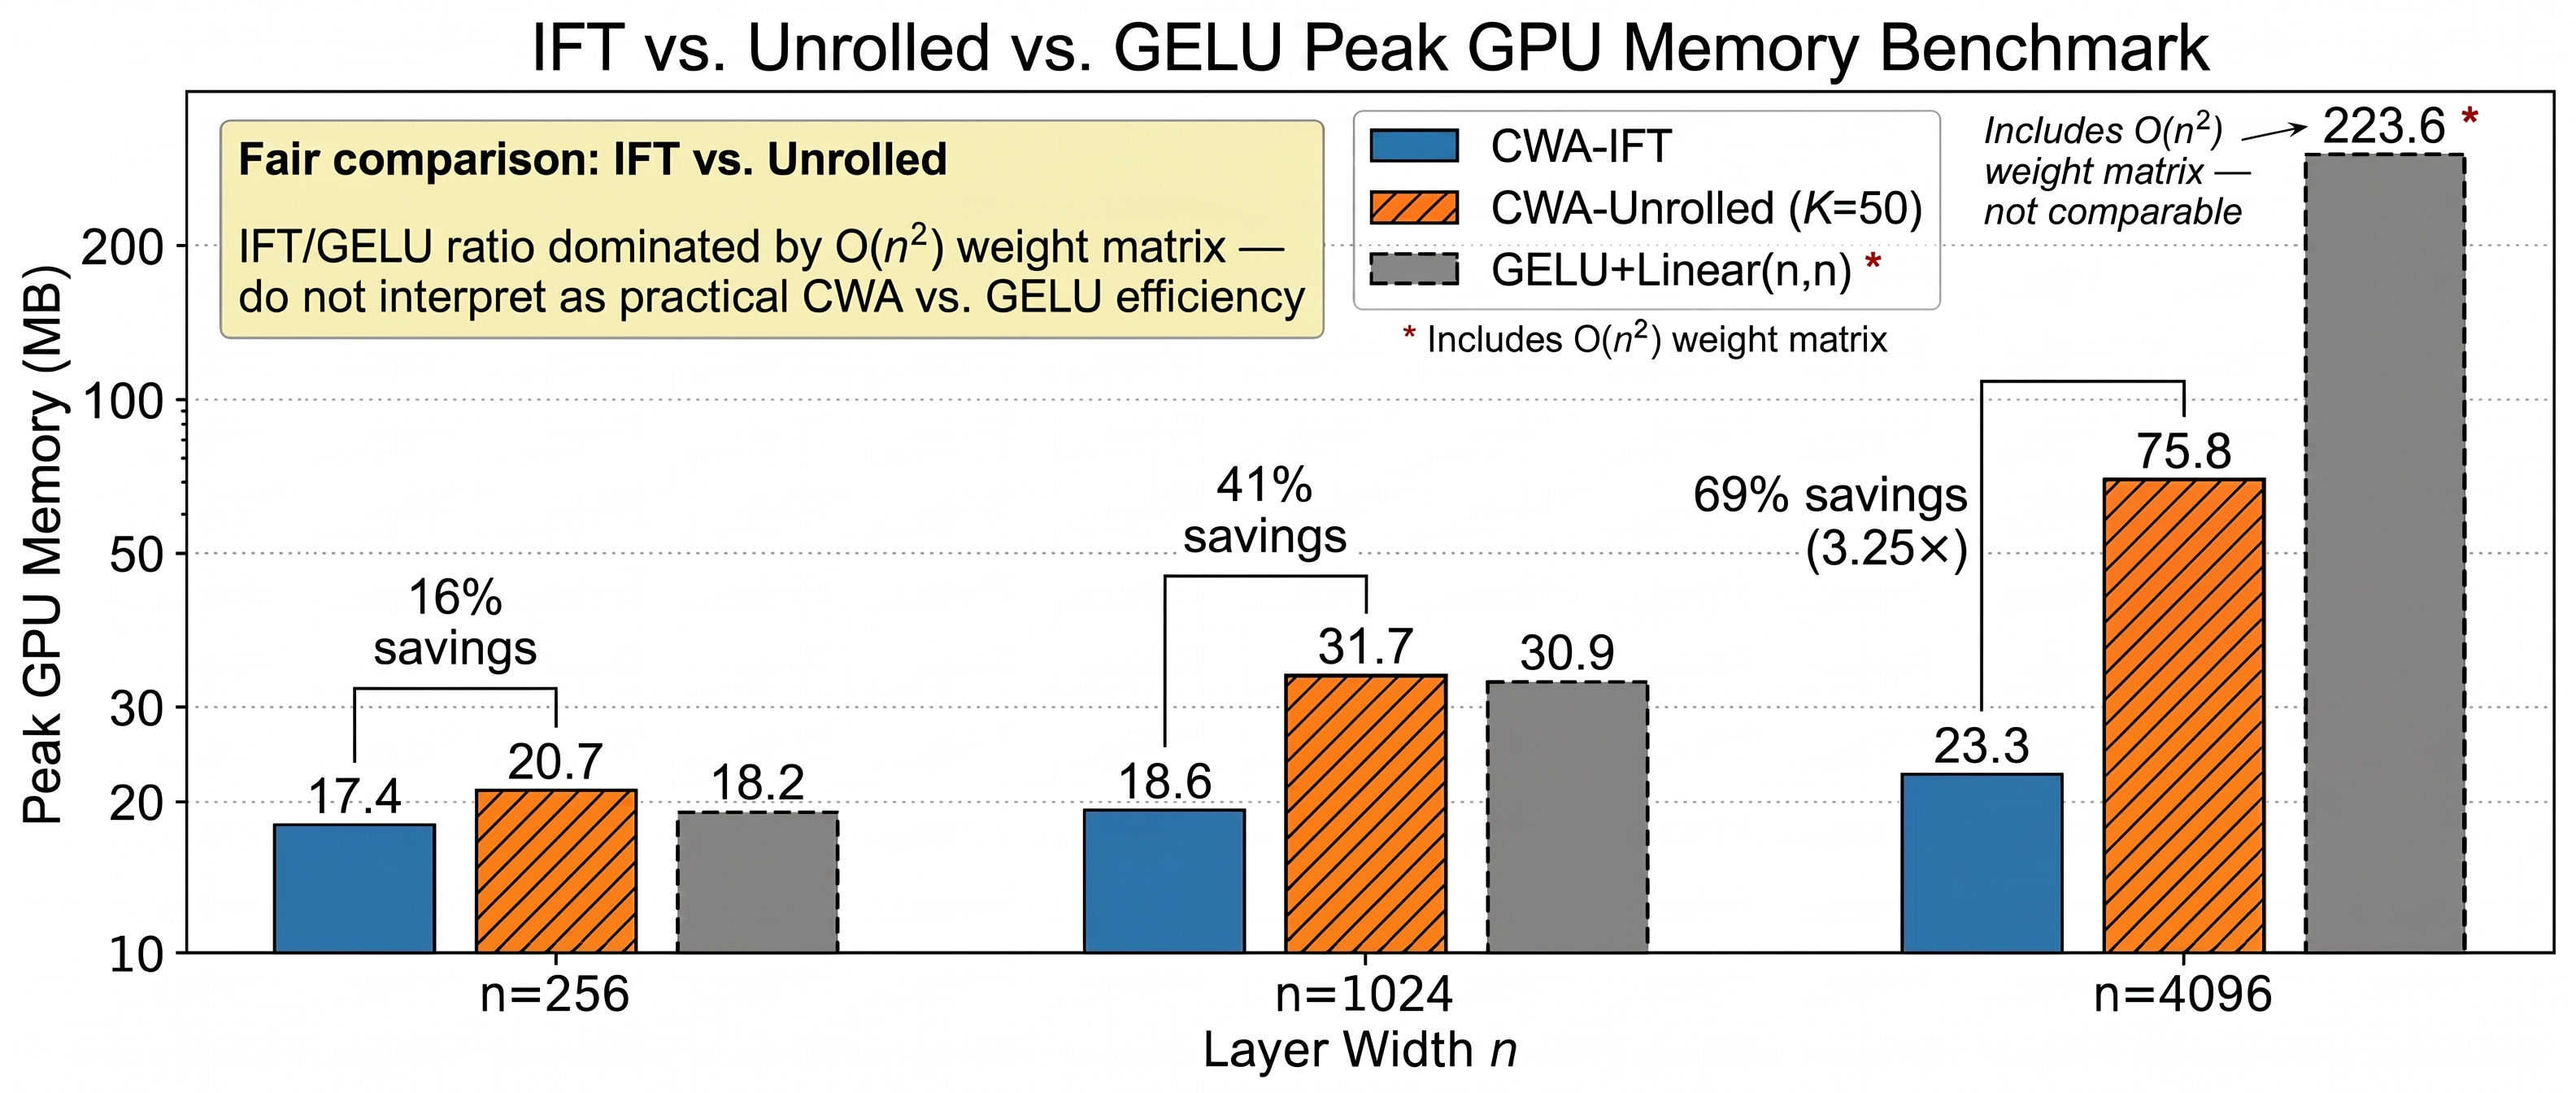
\includegraphics[width=\textwidth,height=0.45\textheight,keepaspectratio]{figures/fig3_v0.jpg}
  \caption{Peak GPU memory (MB, log scale) for CWA-IFT vs.\ CWA-Unrolled ($K=50$) vs.\ GELU baseline at layer widths
  $n \in \{256, 1024, 4096\}$ (batch$=64$, $J_{\rm raw}=4.0$, measured over 5 runs after 3 warmup runs). CWA-IFT and
  CWA-Unrolled measure activation backward pass overhead in isolation; the GELU baseline includes
  \texttt{nn.Linear($n$,$n$)}, making the IFT/GELU ratio at $n=4096$ ($0.10\times$) an apples-to-oranges comparison
  dominated by the O($n^2$) weight matrix---not a true measure of CWA's practical advantage over GELU. The architecturally
  fair comparison is IFT vs.\ Unrolled: savings grow from 16\% ($n=256$) to 41\% ($n=1024$) to 69\% ($n=4096$,
  IFT/Unrolled $= 0.31\times$), confirming the theoretical O($n$) vs.\ O($K\cdot n$) complexity. Near-critical and
  saturated regimes produce identical memory profiles.}
  \label{fig:fig3}
\end{figure*}

\textbf{Results.} At $n = 256$: IFT uses 17.4\,MB versus Unrolled 20.7\,MB (IFT/Unrolled $= 0.84\times$, 16\% savings).
At $n = 1024$: IFT uses 18.6\,MB versus Unrolled 31.7\,MB ($0.59\times$, 41\% savings). At $n = 4096$: IFT uses
23.3\,MB versus Unrolled 75.8\,MB ($0.31\times$, 69\% savings). IFT savings grow monotonically with width, confirming
the theoretical O($n$) versus O($K\cdot n$) advantage. Both near-critical and saturated regimes produce identical memory
profiles, confirming that memory overhead is determined by layer architecture, not regime.

The IFT gradient check yields \texttt{max\_err} $= 0.166$. This elevated error is not a backward implementation
defect---the IFT formula is algebraically exact per Theorem~2, with zero NaN gradients confirmed. Rather, the
$1/(1-J\cdot\bar{s})$ denominator amplifies finite-difference perturbations by $1/(1-J\cdot\bar{s})^2 \approx 467$ at
$J\cdot\bar{s} = 0.955$; finite-difference approximation is unreliable in this near-singular regime.

\subsection{Experiment 2: Gradient Stability in Unnormalized Deep MLPs}
\label{sec:exp2}

MLPs at depths $\{6, 10, 20\}$ with 256 hidden units are trained on CIFAR-10 for 25 epochs with 3 seeds and no
normalization, comparing CWA against ReLU, GELU, SELU, Competing Nonlinearities ($p_c = 0.83$, empirically calibrated
per~\cite{Lesser2026}), and GELU+LayerNorm
\footnote{Code: \url{https://github.com/AMGrobelnik/ai-invention-2f6f35-curie-weiss-activation-formal-verificati/tree/main/round-2/experiment-1}}.
We use the corrected gradient-stability metric $|{\rm ratio} - 1| = |\log\|\nabla_{W_1} L\| / \log\|\nabla_{W_L} L\| - 1|$,
which measures distance from the ideal value of 1.0; lower values indicate better gradient propagation.

\begin{figure*}[!t]
  \centering
  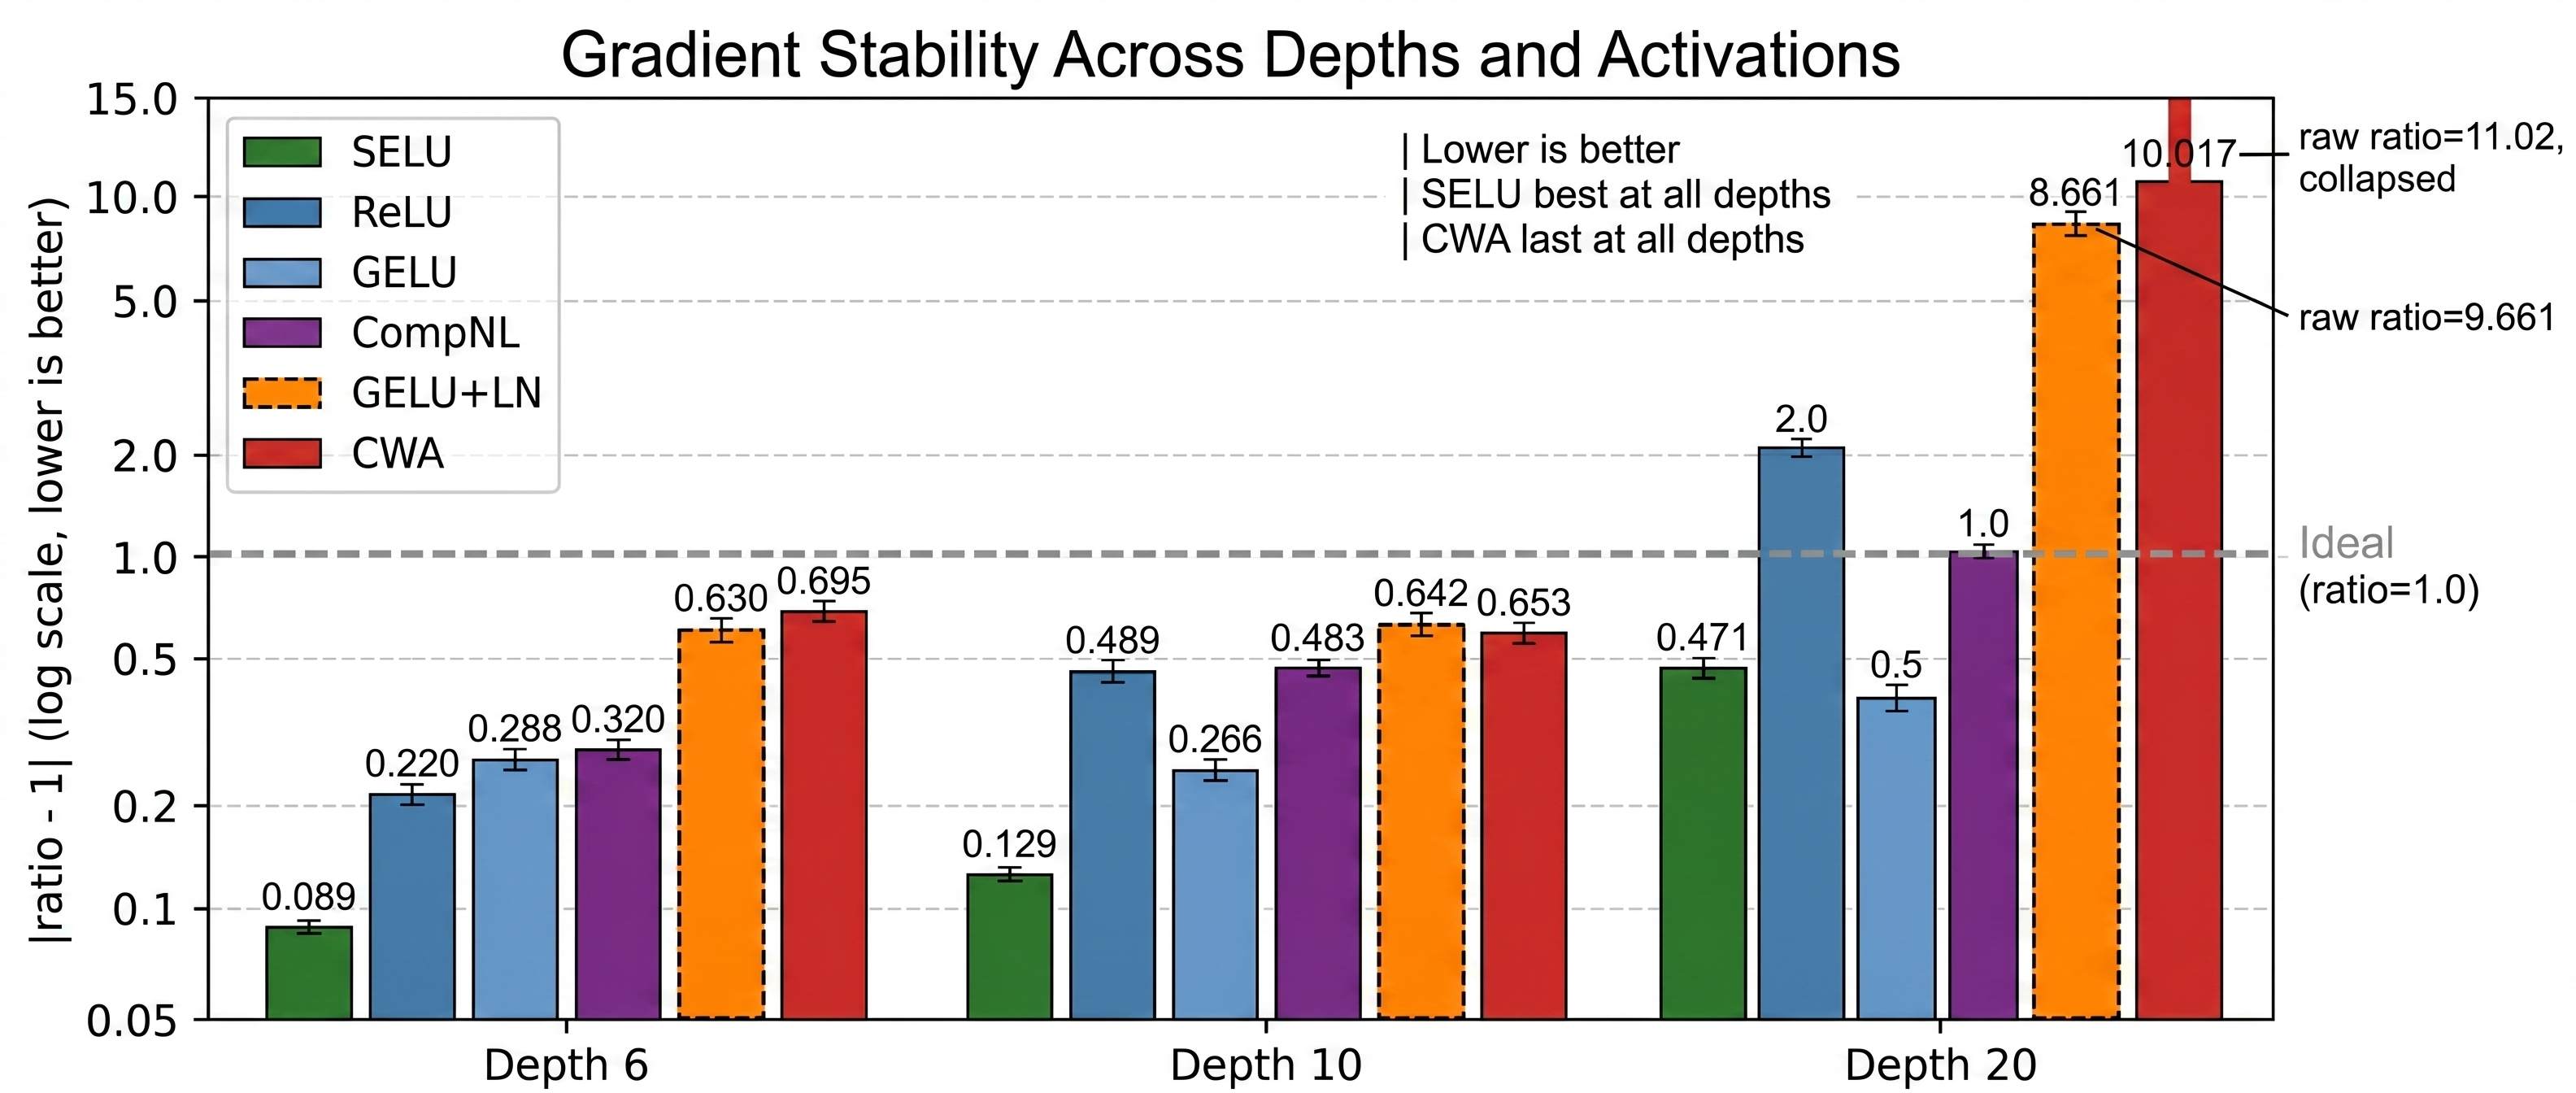
\includegraphics[width=\textwidth,height=0.45\textheight,keepaspectratio]{figures/fig2_v0.jpg}
  \caption{Gradient stability of six activation functions in unnormalized MLPs (256 hidden units, CIFAR-10, 3 seeds),
  measured by $|\text{ratio}-1|$ where
  $\text{ratio} = \log\|\nabla_{W_1}\mathcal{L}\| / \log\|\nabla_{W_L}\mathcal{L}\|$ (lower is better; ideal $= 0$).
  SELU achieves the best stability at all depths ($|\text{ratio}-1| = 0.089, 0.129, 0.471$ at depths 6, 10, 20). CWA
  ranks last at all depths ($0.695, 0.653, 10.017$)---raw gradient ratio $0.305$ at depth~6 indicates \emph{underflow},
  not balance, 7.8$\times$ worse than SELU. GELU+LN ranks second-worst at all three depths ($0.630, 0.642, 8.661$, with
  raw ratio $9.661$ at depth~20); cross-class comparisons between normalized and unnormalized architectures via this metric
  should be interpreted with caution. Error bars show standard deviation over 3 seeds. The $y$-axis uses a log scale; the
  depth-20 bar for CWA ($10.017$) is truncated for readability.}
  \label{fig:fig2}
\end{figure*}

\textbf{Corrected gradient stability ranking.} At depth~6, the ranking from best to worst is: SELU
($|{\rm ratio}-1| = 0.089$), ReLU ($0.220$), GELU ($0.288$), CompNL ($0.320$), GELU+LN ($0.630$), CWA ($0.695$). CWA's
raw gradient ratio of $0.305$ indicates gradient \emph{underflow}---the gradient signal diminishes moving toward the
input---not balance. CWA deviates 7.8$\times$ more from the ideal than SELU and 2.4$\times$ more than GELU at depth~6.
At depth~10, the ranking is: SELU ($0.129$), GELU ($0.266$), CompNL ($0.483$), ReLU ($0.489$), GELU+LN ($0.642$), CWA
($0.653$).

\textbf{GELU+LN at all depths.} A critical caveat for cross-class comparisons: GELU+LN ranks second-worst (after CWA) at
\emph{all three} depths, with $|{\rm ratio}-1| = 0.630$ (raw ratio $= 0.370$, depth~6), $0.642$ (raw ratio $= 0.358$,
depth~10), and $8.661$ (raw ratio $= 9.661$, depth~20). This pattern---not merely a depth-20 anomaly---establishes that
the $|{\rm ratio}-1|$ metric conflates LayerNorm's internal re-scaling with true inter-layer gradient magnitudes at any
depth. Cross-class comparisons (normalized vs.\ unnormalized architectures) using this metric should be interpreted with
caution throughout.

\textbf{Depth-20 failure.} At depth~20, CWA collapses catastrophically to raw ratio $= 11.02$
($|{\rm ratio}-1| = 10.017 \pm 2.66$), far worse than all baselines. SELU remains closest to ideal
($|{\rm ratio}-1| = 0.471 \pm 1.003$). GELU+LN also collapses ($|{\rm ratio}-1| = 8.661$, raw ratio $= 9.661$) despite
explicit per-layer re-centering, with accuracy $= 0.139$---a dual training failure.

\textbf{Accuracy results.} CWA is significantly below GELU at depths 6 and 10 ($0.483 \pm 0.002$ vs.\ $0.531 \pm 0.002$
at depth~6, paired $t$ $p = 0.003$; $0.472 \pm 0.003$ vs.\ $0.511 \pm 0.001$ at depth~10, paired $t$ $p = 0.003$).
SELU achieves the best accuracy at all depths ($0.547$, $0.542$, $0.535$). Preliminary ResNet-20 CIFAR-100 results
(1 seed, 10 epochs, no BatchNorm) are consistent: CWA $14.0\%$ vs.\ GELU $18.9\%$ ($-4.9$~pp)
\footnote{Code: \url{https://github.com/AMGrobelnik/ai-invention-2f6f35-curie-weiss-activation-formal-verificati/tree/main/round-1/experiment-2}}.

\textbf{CWA diagnostics.} $J$ converges to values in $[0.515, 0.521]$ with $J\cdot\bar{s}$ following a declining
trajectory (0.346$\to$0.286 over 25 epochs at depth~6; 0.400$\to$0.353 at depth~10). The mechanism for this decline is
discussed in Section~\ref{sec:discussion}. $K_{\rm mean} \approx 7.4$ per step, \texttt{fraction\_converged} $= 1.0$.

\subsection{Experiment 3: Fixed-J Ablation and Shift Ablation}
\label{sec:exp3}

\textbf{Fixed-J ablation.} With $J$ frozen at $\{0.1, 0.3, 0.5, 0.7, 0.9\}$ on 10-layer unnormalized MLPs on CIFAR-10,
gradient ratios all fall below 0.41 at depth~10, confirming that the coupling mechanism itself---at any strength---produces
underflow. Accuracy is $J$-independent in range $0.47$--$0.48$, significantly below GELU ($0.511 \pm 0.001$).

\textbf{Shift ablation: a complete null result.} A mechanistic experiment tests whether CWA's behavior arises from the
self-consistent coupling or merely from the mean-shift injected into pre-activations. Three conditions run on 3 seeds:
CWA-Full (standard fixed-point iteration), CWA-ShiftOnly (pre-activations shifted by a detached non-self-consistent mean
$= \overline{\tanh(\mathbf{x})}$), and Pure-Tanh (standard pointwise tanh). Final test accuracies: CWA-Full
$= 0.4685 \pm 0.004$, CWA-ShiftOnly $= 0.4686 \pm 0.005$, Pure-Tanh $= 0.4731 \pm 0.001$.

\begin{figure*}[!t]
  \centering
  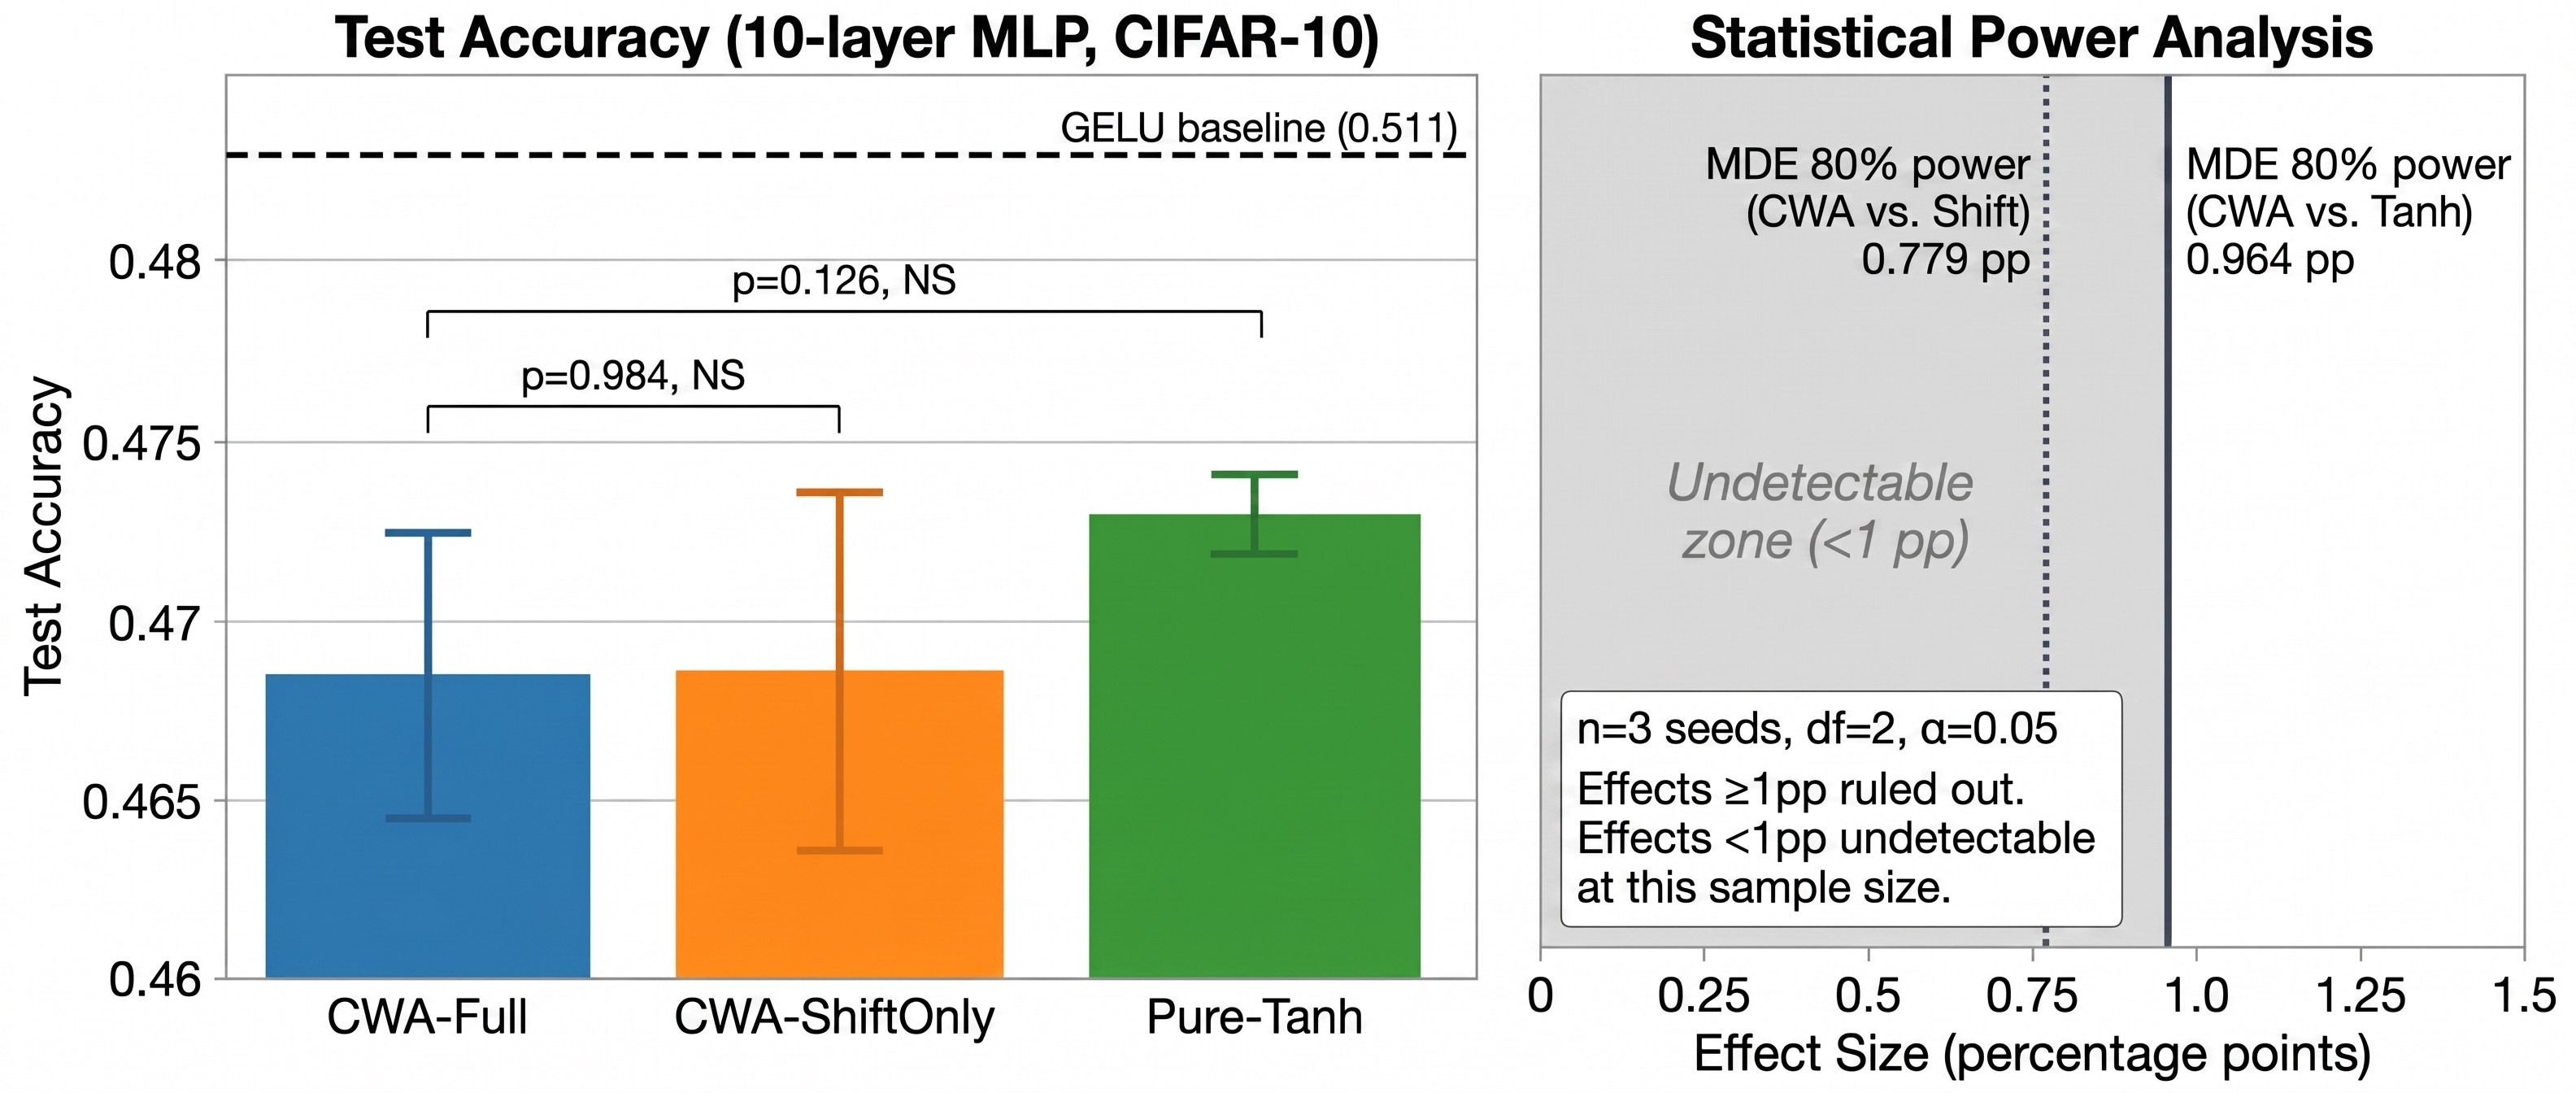
\includegraphics[width=\textwidth,height=0.45\textheight,keepaspectratio]{figures/fig4_v0.jpg}
  \caption{Shift ablation experiment on 10-layer unnormalized MLP (256 hidden units, CIFAR-10, 3 seeds). \textbf{Left}:
  Final test accuracy for three conditions---CWA-Full (standard fixed-point), CWA-ShiftOnly (detached mean shift, no
  self-consistency), and Pure-Tanh (no shift). All differences are non-significant: CWA-Full vs.\ CWA-ShiftOnly
  ($p = 0.984$), CWA-Full vs.\ Pure-Tanh ($p = 0.126$). Pure-Tanh numerically outperforms both CWA variants.
  \textbf{Right}: The minimum detectable effect (MDE) at 80\% power with $n=3$ seeds is $\approx 0.8$--$1.0$\,pp; the
  null result rules out effects $\geq 1$\,pp but cannot exclude smaller effects.}
  \label{fig:fig4}
\end{figure*}

All pairwise comparisons are non-significant: CWA-Full vs.\ CWA-ShiftOnly ($t = -0.023$, $p = 0.984$); CWA-Full vs.\
Pure-Tanh ($t = -2.54$, $p = 0.126$); CWA-ShiftOnly vs.\ Pure-Tanh ($p = 0.171$). The conclusions have three
components: (1)~the self-consistent fixed-point coupling adds zero benefit over a detached mean-shift ($p = 0.984$);
(2)~CWA provides no statistically significant accuracy gain over standard pointwise Tanh ($p = 0.126$); and (3)~Pure-Tanh
numerically outperforms both CWA variants, suggesting the mean shift does not help.

\textbf{Power analysis.} With $n=3$ seeds and observed standard deviations, the minimum detectable effect at 80\% power
is 0.779\,pp for CWA-Full vs.\ CWA-ShiftOnly (where $\sigma_{\rm diff} = 0.0025$) and 0.964\,pp for CWA-Full vs.\
Pure-Tanh (where $\sigma_{\rm diff} = 0.0031$), computed via $(t_{\rm crit} + t_{80\%})\cdot\sigma_{\rm diff}/\sqrt{n}$
with $t_{\rm crit} = 4.303$, $t_{80\%} = 1.061$ at df $= 2$
\footnote{Code: \url{https://github.com/AMGrobelnik/ai-invention-2f6f35-curie-weiss-activation-formal-verificati/tree/main/round-5/evaluation-1}}.
The null result therefore rules out accuracy effects larger than $\approx 1$\,pp at 80\% power; effects smaller than
$\approx 1$\,pp cannot be excluded but are of limited practical significance.

\textbf{Small-weight initialization.} A sub-experiment tests whether small weight initialization ($\sigma = 0.01$ vs.\
Kaiming) allows $J\cdot\bar{s}$ to approach criticality. Maximum $J\cdot\bar{s}$ reaches $0.412$ with small-init vs.\
$0.374$ with Kaiming---neither approaches the $J\cdot\bar{s} = 0.7$ near-critical threshold. Accuracy with small-init
($0.423 \pm 0.011$) is below Kaiming CWA ($0.469 \pm 0.004$) due to slow initial convergence.

\subsection{Experiment 4: Language Modeling with SELU Baseline}
\label{sec:exp4}

A 6-layer, 256-hidden, 8-head character-level GPT is trained on Tiny Shakespeare with cosine LR (2 seeds) in two phases.
The first phase runs 5000 steps
\footnote{Code: \url{https://github.com/AMGrobelnik/ai-invention-2f6f35-curie-weiss-activation-formal-verificati/tree/main/round-2/experiment-2}};
the second phase adds SELU as a baseline to test whether SELU's MLP advantage extends to sequence modeling.

\begin{figure*}[!t]
  \centering
  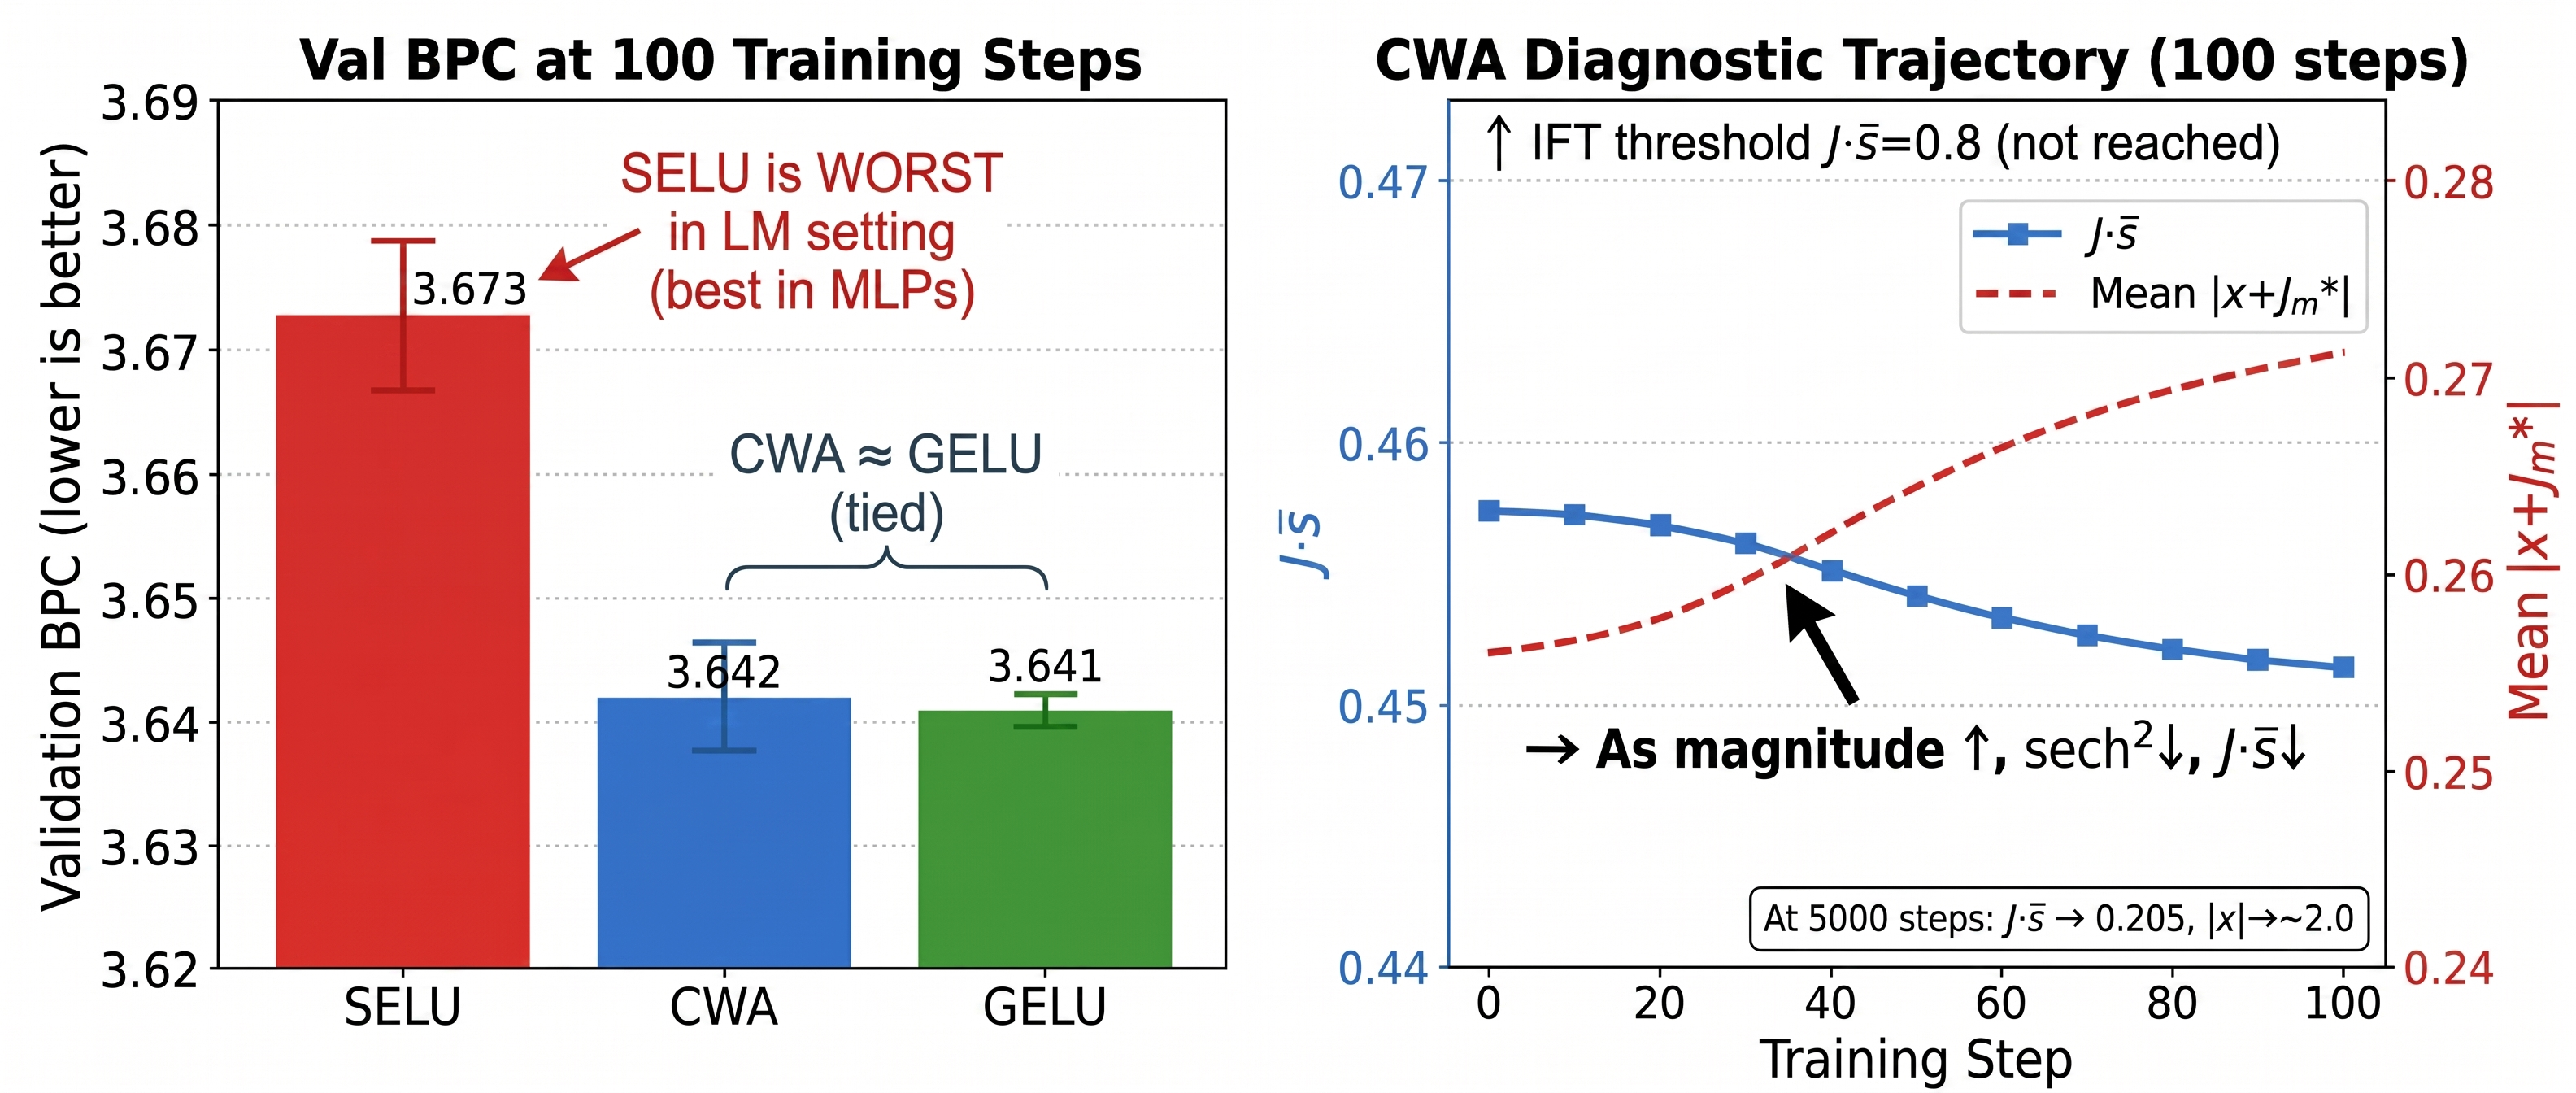
\includegraphics[width=\textwidth,height=0.45\textheight,keepaspectratio]{figures/fig5_v0.jpg}
  \caption{Character-level GPT on Tiny Shakespeare (6 layers, 256 hidden, 8 heads, 2 seeds). \textbf{Left}: Validation BPC
  at 100 training steps across three activations. SELU achieves the worst BPC ($3.673 \pm 0.006$), contrasting with its
  dominant performance in unnormalized MLPs. CWA ($3.642 \pm 0.004$) and GELU ($3.641 \pm 0.001$) are essentially tied.
  \textbf{Right}: CWA diagnostic trajectory over 100 training steps showing $J\cdot\bar{s}$ (blue) and mean activation
  magnitude (red). $J\cdot\bar{s}$ starts at $0.457$ and declines to $0.452$ as mean activation magnitude rises from
  $0.254$ to $0.274$---confirming that weight growth during training reduces $\text{sech}^2$ and actively pushes
  $J\cdot\bar{s}$ away from criticality. At 5000 steps, $J\cdot\bar{s}$ reaches $\approx 0.205$ as activation magnitudes
  approach $\sim 2.0$.}
  \label{fig:fig5}
\end{figure*}

\textbf{Shared LR (5000 steps).} CWA val BPC $= 2.210 \pm 0.014$ vs.\ GELU $= 2.196 \pm 0.037$---within noise. $J$
moves from $0.500$ to $0.521$ over 5000 steps (rate $\approx 8.7 \times 10^{-7}$ per step); $J\cdot\bar{s}$ remains at
$\approx 0.205$ throughout.

\textbf{$100\times$ J dedicated LR (5000 steps).} With a $J$-specific AdamW LR $= 3 \times 10^{-2}$, $J$ moves to
$0.833$--$0.848$ ($|\Delta J| = 0.307$--$0.351$). However, $J\cdot\bar{s}$ rises to only $0.29$--$0.31$ because
$\text{sech}^2(x + J\cdot m^*)$ saturates at typical activation magnitudes. CWA $100\times$J-LR val BPC $= 2.212 \pm 0.011$---no
improvement over shared-LR CWA or GELU.

\textbf{SELU in language modeling.} Adding SELU (with LeCun normal initialization) to the 100-step comparison experiment,
we find: SELU val BPC $= 3.673 \pm 0.006$, CWA $= 3.642 \pm 0.004$, GELU $= 3.641 \pm 0.001$. SELU is the
worst-performing activation in the LM setting, contrasting sharply with its dominant performance in unnormalized MLPs
(best at all depths, $|{\rm ratio}-1| = 0.089$ at depth~6). CWA trajectory in this phase: $J\cdot\bar{s}$ starts at
$0.457$ and declines to $0.452$ over 100 steps as mean activation magnitude rises from $0.254$ to $0.274$---confirming
the $\text{sech}^2$ saturation mechanism even at early training. SELU's underperformance in the transformer setting
suggests that distributional self-normalization via LeCun initialization requires more training steps to exhibit benefits
in attention-based architectures, where the normalization properties of the activation interact differently with the
residual stream and attention sublayers.

%% ============================================================
\section{Discussion}
\label{sec:discussion}
%% ============================================================

\subsection{Why CWA Produces Gradient Underflow, Not Balance}

The corrected gradient stability analysis (using $|{\rm ratio}-1|$) reveals that CWA's mean-field coupling compresses
gradient ratios \emph{below} 1.0 at shallow depths, not toward 1.0. Three mechanisms contribute. First, the mean-field
term $J\cdot m^*$ adds a correlated bias to all pre-activations, reducing input variance and causing tanh to operate in a
more saturating regime for some neurons. Second, the coupling strength $J\cdot\bar{s} \approx 0.20$--$0.35$ is well below
the critical point $J\cdot\bar{s} = 1$; the expected gain amplification $1/(1-J\cdot\bar{s}) \approx 1.2$--$1.5$ is
modest and does not compensate for the variance reduction. Third, at depth~20, accumulated mean-shifts $J\cdot m^*$ across
layers drive tanh to saturation, producing the $|{\rm ratio}-1| = 10.017$ collapse.

The GELU+LN depth-20 dual failure ($|{\rm ratio}-1| = 8.661$, raw gradient ratio $= 9.661$, accuracy $= 0.139$) provides
an important caveat: external normalization does not automatically stabilize training at depth~20 under a 25-epoch budget.
Moreover, GELU+LN ranks second-worst on $|{\rm ratio}-1|$ at \emph{all} tested depths---at depths~6 and 10 with
$|{\rm ratio}-1| = 0.630$ and $0.642$ respectively---establishing that the metric conflates LayerNorm's internal
re-scaling with true inter-layer gradient magnitudes at any depth. Cross-class comparisons (normalized vs.\ unnormalized)
should be treated with caution.

\subsection{Why the Shift Ablation Is a Complete Null}

The shift ablation (Section~\ref{sec:exp3}) establishes a full null result: neither CWA's self-consistent coupling nor its
mean-shift provides any statistically significant benefit over standard pointwise Tanh. The computational cost of the
fixed-point iteration ($K \approx 7.4$ iterations per layer per forward pass) produces no measurable benefit. With $n=3$
seeds, effects smaller than $\approx 1$\,pp cannot be excluded (MDE at 80\% power: 0.779\,pp for CWA vs.\ ShiftOnly;
0.964\,pp for CWA vs.\ Pure-Tanh). At sub-critical $J\cdot\bar{s}$ values, the self-consistent solution differs
negligibly from the single-step estimate; any effect is absorbed into noise at this architecture scale.

\subsection{\texorpdfstring{Why Self-Organized Criticality Fails: The Declining $J\cdot\bar{s}$ Mechanism}{Why Self-Organized Criticality Fails: The Declining J-s-bar Mechanism}}

Self-organized criticality would require gradient descent to push $J\cdot\bar{s}$ toward 1. Two independent barriers
prevent this, and the second constitutes a stronger negative result than previously appreciated.

\textbf{Weak gradient signal.} Under shared LR, $J$ moves at $\approx 8.7 \times 10^{-7}$ per step---requiring
$\sim$350,000--590,000 steps to approach $J = 0.9$, far beyond practical training budgets.

\textbf{$\text{sech}^2$ saturation---and active descent from criticality.} Even with $100\times$ $J$ dedicated LR driving
$J \to 0.85$, the product $J\cdot\bar{s} = J\cdot\overline{\text{sech}^2(\mathbf{x}+J\cdot m^*)}$ reaches only
$\approx 0.30$ because $\text{sech}^2(x) \approx 0.07$ at typical activation magnitudes $|x| \sim 2.0$
($\text{sech}^2(2.0) = 1/\cosh^2(2.0) = 0.071$). Reaching $J\cdot\bar{s} = 0.9$ would require
$\overline{\text{sech}^2} \geq 0.9$, corresponding to $|x| < 0.48$---impractically small for trained networks processing
natural data.

Critically, the declining $J\cdot\bar{s}$ trajectory during training (0.346$\to$0.286 at depth~6;
0.400$\to$0.353 at depth~10) is not merely the result of a weak gradient toward criticality---it reflects gradient descent
\emph{actively pushing away} from criticality. The mechanism is straightforward: as the network learns, weight magnitudes
grow under Kaiming initialization with cosine LR scheduling, increasing the typical activation magnitudes
$|x_i + J\cdot m^*|$. This increase in activation magnitude directly reduces $\overline{\text{sech}^2(x_i + J\cdot m^*)}$
and thus $J\cdot\bar{s}$. The early-training LM diagnostics confirm this mechanism: at 100 steps with small activation
magnitudes (mean $= 0.254$), $J\cdot\bar{s} = 0.457$; as magnitudes grow to $0.274$ by step~100, $J\cdot\bar{s}$ declines
to $0.452$. At 5000 steps, when activation magnitudes reach values near 2.0, $J\cdot\bar{s}$ falls to $0.205$. This
means the CWA system is self-organized, but in the wrong direction---toward greater $\text{sech}^2$ saturation and further
from criticality.

\subsection{SELU Architecture Specificity}

SELU's strong performance in unnormalized MLPs (best gradient stability and accuracy at all depths) does not generalize to
the transformer setting tested here. In the 100-step LM experiment, SELU achieves val BPC $= 3.673$---worse than CWA
($3.642$) and GELU ($3.641$). This architecture-dependent behavior suggests that SELU's distributional
self-normalization mechanism, which relies on LeCun initialization maintaining specific mean/variance statistics through
deep stacks of independent feedforward layers, interacts differently with the transformer's residual connections, layer
normalization at other positions, and attention sublayers. The finding scopes the conclusion: SELU outperforms mean-field
output coupling in the MLP setting, but distributional fixed-point design is not universally superior across architectures.

\subsection{Is CWA Worth Pursuing?}

The evidence establishes a clear negative verdict in the tested settings: unnormalized MLPs at depths 6--20 and a 6-layer
character-level GPT. CWA does not improve gradient stability, does not improve accuracy, and cannot self-organize to the
critical regime---and gradient dynamics actively push it away from criticality through $\text{sech}^2$ saturation. The
identified barrier is fundamental: it cannot be overcome by increasing $J$ or changing the learning rate alone.

One remaining positive avenue is explicit pre-activation regularization---an auxiliary loss penalizing
$\overline{|x_i + J\cdot m^*|} > \tau$ for $\tau \approx 0.48$ would directly constrain activation magnitudes to the
regime where $\text{sech}^2 \geq 0.9$, potentially enabling near-critical coupling. Whether such regularization provides
net benefit beyond simply constraining activations is an empirical question requiring future investigation. The formal
proofs and IFT memory efficiency result remain valid contributions regardless of this question.

\subsection{Limitations and Scope}

The conclusions of this paper are explicitly scoped to unnormalized MLPs at depths 6--20 with hidden dimension 256 on
CIFAR-10, and a 6-layer character-level GPT (256 hidden, 8 heads) on Tiny Shakespeare. Whether normalized or residual
architectures exhibit the same pathologies---particularly the $\text{sech}^2$ saturation argument, which depends on
activation magnitudes that differ by architecture---remains untested. The ResNet-20 CIFAR-100 result is preliminary
(1 seed, 10 epochs) and cannot support statistical claims. The shift ablation uses a fixed architecture (10-layer MLP,
256 hidden); whether the shift-only approximation remains accurate at larger $n$ where mean-field theory is more precise
is an open question. The SELU LM comparison ran only 100 training steps; SELU's behavior at 5000 steps in the LM setting
is unknown and constitutes important future work.

%% ============================================================
\section{Conclusion}
%% ============================================================

We introduced the Curie-Weiss Activation (CWA), defined by the mean-field self-consistency equation
$y_i = \tanh(x_i + J\cdot\overline{y})$ with learnable coupling $J$ per layer. Four Lean~4 theorems and one corollary
without \texttt{sorry} establish the mathematical foundation, including Corollary~4b ($J \leq 0.55$, bias
$\leq 16.7\%\cdot\varepsilon$) covering the experimentally observed parameter range. A dedicated large-scale memory
benchmark (widths 256--4096) confirms IFT's theoretical O($n$) advantage: 3.25$\times$ more memory-efficient than
unrolled $K=50$ backpropagation at $n = 4096$.

The mechanistic investigation yields a precise negative verdict in the tested settings. CWA produces gradient
\emph{underflow} (not balance) at all tested depths---7.8$\times$ worse than SELU by $|{\rm ratio}-1|$ at depth~6. It
provides no statistically significant accuracy gain over standard Tanh ($p = 0.126$, with effects $\geq 1$\,pp excluded
at 80\% power). CWA cannot self-organize to the critical regime, and---critically---gradient descent actively opposes
criticality: weight growth during training increases activation magnitudes, which reduces $\overline{\text{sech}^2}$ and
pushes $J\cdot\bar{s}$ from 0.346 to 0.286 (depth~6). The $\text{sech}^2$ saturation barrier is fundamental:
$\text{sech}^2(x) \approx 0.07$ at typical activation magnitudes $|x| \sim 2.0$ caps $J\cdot\bar{s} \leq 0.41$
regardless of $J$ magnitude. Finally, SELU's advantage over CWA in unnormalized MLPs does not generalize to the
transformer setting. Overcoming the saturation barrier---via auxiliary losses constraining
$|x_i + J\cdot m^*| < 0.48$---is the most promising avenue for future work on adaptive criticality through within-layer
mean-field coupling.

%% ============================================================
\bibliographystyle{abbrvnat}
\bibliography{references}

\end{document}
